% =====================================================================
%  ANEXOS
% =====================================================================
\chapter{Detalle de los temas detectados}
\label{anexo:topics}

Este anexo recoge el detalle completo de los veinticinco temas identificados por el modelo LDA,
con sus palabras características, la etiqueta interpretativa asignada y su correspondencia
aproximada con los estándares ESRS (tabla~\ref{tab:lda-full}). Complementa la agrupación en
siete bloques presentada en la sección~\ref{sec:res-temas}.

\begin{longtable}{p{0.8cm}p{6.4cm}p{4.6cm}p{1.4cm}}
\caption{Temas del modelo LDA ($K=25$) con etiquetas interpretativas}
\label{tab:lda-full}\\
\toprule
\textbf{Tema} & \textbf{Palabras características} & \textbf{Etiqueta} & \textbf{ESRS} \\
\midrule
\endfirsthead
\multicolumn{4}{c}{\tablename\ \thetable\ -- \textit{continuación}}\\
\toprule
\textbf{Tema} & \textbf{Palabras características} & \textbf{Etiqueta} & \textbf{ESRS} \\
\midrule
\endhead
\midrule
\multicolumn{4}{r}{\textit{continúa en la página siguiente}}\\
\endfoot
\bottomrule
\endlastfoot
T00 & waste, products, materials, use, product, circular, economy & Economía circular y residuos & E5 \\
T01 & requirements, regulations, standards, companies, compliance, regulatory & Marco normativo general & ESRS 2 \\
T02 & compliance, conduct, code, corruption, ethics, policy, employees & Ética y anticorrupción & G1 \\
T03 & stakeholders, engagement, survey, dialogue, stakeholder, industry & Diálogo con grupos de interés & ESRS 2 \\
T04 & sustainable, development, strategy, commitment, people, culture & Estrategia y compromiso & ESRS 2 \\
T05 & investment, portfolio, financial, assets, investments, capital & Inversión y activos financieros & --- \\
T06 & risk, management, internal, process, risks, measures, system & Sistemas de gestión de riesgos & ESRS 2 / G1 \\
T07 & activities, taxonomy, eligible, aligned, economic, activity, capex & Taxonomía de la UE & --- \\
T08 & targets, target, carbon, climate, transition, zero, plan & Metas climáticas y transición & E1 \\
T09 & due, could, increased, increase, market, costs, changes & Lenguaje de riesgo financiero & --- \\
T10 & risks, climate, impacts, opportunities, material, related, risk & Doble materialidad & ESRS 2 \\
T11 & new, training, development, support, program, learning, digital & Formación y desarrollo del talento & S1 \\
T12 & sustainability, performance, esg, strategy, environmental, governance & Desempeño ESG & ESRS 2 \\
T13 & water, sites, production, air, site, consumption, pollution & Agua, aire y contaminación & E2 / E3 \\
T14 & employees, health, safety, employee, work, diversity, workforce & Salud, seguridad y diversidad & S1 \\
T15 & board, committee, executive, directors, members, remuneration & Gobierno corporativo & G1 \\
T16 & energy, consumption, hydro, renewable, electricity, efficiency, gas & Energía y eficiencia energética & E1 \\
T17 & data, services, customers, customer, security, service, products & Productos, clientes y ciberseguridad & S4 \\
T18 & reporting, esrs, financial, gri, sustainability, statements, disclosure & Marco de reporting ESRS/GRI & ESRS 2 \\
T19 & million, share, net, revenue, income, per, december & Métricas financieras & --- \\
T20 & years, france, first, europe, two, spain, germany & Geografía y contexto internacional & --- \\
T21 & biodiversity, environmental, impact, impacts, areas, communities, local & Biodiversidad y comunidades & E4 / S3 \\
T22 & emissions, scope, ghg, data, emission, gas, greenhouse & Emisiones de gases de efecto invernadero & E1 \\
T23 & human, rights, labour, principles, workers, labor, due & Derechos humanos y debida diligencia & S2 \\
T24 & chain, suppliers, value, supply, supplier, procurement & Cadena de suministro y proveedores & S2 \\
\end{longtable}
{\footnotesize Fuente: elaboración propia a partir del modelo LDA.}

\bigskip
Por su parte, el modelo BERTopic identificó 578 temas, de los que aproximadamente el 40\,\% de
los párrafos quedó sin clasificar. Entre los temas más frecuentes destacan el riesgo climático
físico, el gobierno corporativo, la cadena de suministro, la gestión del agua, la biodiversidad,
la diversidad de género, la salud y seguridad laboral, la doble materialidad, la Taxonomía de la
UE y la ciberseguridad, junto a numerosos temas específicos de empresas concretas. La
coincidencia de estos grandes temas con los del modelo LDA constituye la base de la triangulación
discutida en la sección~\ref{sec:res-temas}.

\chapter{Resultados completos de las regresiones}
\label{anexo:regresiones}

Este anexo recoge los coeficientes completos de las dos regresiones por mínimos cuadrados
ordinarios con errores estándar robustos a la heterocedasticidad (HC3) presentadas de forma
resumida en la sección~\ref{sec:res-determinantes}. Las categorías de referencia son el sector
de materiales básicos, el año 2022 y la región centro. La estimación se realizó sobre 577
observaciones. El factor de inflación de la varianza se mantuvo por debajo de 3 en todos los
predictores de ambos modelos, lo que descarta problemas relevantes de multicolinealidad.

\begin{table}[H]
\centering
\caption{Regresión 1 --- Variable dependiente: índice de \textit{greenwashing} ($R^2\approx0{,}14$)}
\label{tab:reg1-full}
\begin{tabular}{lrr}
\toprule
\textbf{Predictor} & \textbf{Coef.} & \textbf{$p$} \\
\midrule
Constante & $-$0,401 & 0,813 \\
Communication Services & +0,153 & 0,654 \\
Consumer Discretionary & +0,469 & 0,108 \\
Consumer Staples & +0,582 & 0,169 \\
Energy & +0,443 & 0,206 \\
Financials & +2,034 & $<$0,001 \\
Health Care & +0,519 & 0,250 \\
Industrials & +0,489 & 0,211 \\
Real Estate & $-$0,332 & 0,461 \\
Technology & +1,338 & 0,002 \\
Utilities & $-$0,070 & 0,902 \\
Año 2023 & $-$0,010 & 0,969 \\
Año 2024 & +0,510 & 0,030 \\
Región Nórdicos & +0,612 & 0,022 \\
Región Otros & +3,767 & 0,378 \\
Región Sur & $-$0,505 & 0,150 \\
Región Reino Unido e Irlanda & +0,751 & 0,003 \\
Capitalización (log) & $-$0,026 & 0,723 \\
ROA & +1,445 & 0,192 \\
Deuda/fondos propios & +0,016 & 0,735 \\
\bottomrule
\end{tabular}
\\[4pt]
{\footnotesize Fuente: elaboración propia.}
\end{table}

\begin{table}[H]
\centering
\caption{Regresión 2 --- Variable dependiente: tono financiero (FinBERT) ($R^2\approx0{,}16$)}
\label{tab:reg2-full}
\begin{tabular}{lrr}
\toprule
\textbf{Predictor} & \textbf{Coef.} & \textbf{$p$} \\
\midrule
Constante & +0,135 & 0,244 \\
Communication Services & $-$0,046 & 0,028 \\
Consumer Discretionary & $-$0,002 & 0,923 \\
Consumer Staples & $-$0,011 & 0,666 \\
Energy & $-$0,075 & 0,021 \\
Financials & $-$0,010 & 0,623 \\
Health Care & +0,049 & 0,243 \\
Industrials & +0,000 & 0,983 \\
Real Estate & $-$0,069 & $<$0,001 \\
Technology & $-$0,010 & 0,783 \\
Utilities & $-$0,048 & 0,077 \\
Año 2023 & $-$0,005 & 0,734 \\
Año 2024 & $-$0,048 & $<$0,001 \\
Región Nórdicos & $-$0,011 & 0,533 \\
Región Otros & $-$0,288 & 0,497 \\
Región Sur & +0,009 & 0,606 \\
Región Reino Unido e Irlanda & +0,064 & $<$0,001 \\
Especificidad climática & +0,194 & 0,003 \\
Capitalización (log) & +0,000 & 0,938 \\
ROA & +0,100 & 0,488 \\
\bottomrule
\end{tabular}
\\[4pt]
{\footnotesize Fuente: elaboración propia.}
\end{table}

\chapter{Reproducibilidad: pipeline, software y repositorio}
\label{anexo:reproducibilidad}

Este anexo reúne el detalle técnico necesario para reproducir el trabajo de principio a fin,
en cumplimiento de lo anunciado en la sección~\ref{sec:reproducibilidad}. Se documentan el
pipeline completo, las versiones del software, los parámetros de los modelos y los criterios de
limpieza, y se ofrece la dirección del repositorio público que contiene todo el código.

\section*{Pipeline completo}

El procesamiento se organiza como una secuencia de scripts en Python, encadenados de forma que
la salida de cada fase es la entrada de la siguiente:

\begin{enumerate}
    \item \textbf{Muestra.} Muestreo estratificado por sector sobre el STOXX Europe 600 (semilla
    aleatoria fija) y recopilación de los datos financieros de control desde Yahoo Finance.
    \item \textbf{Recolección.} Descarga de los informes corporativos en PDF y verificación de
    contenido (empresa correcta, tipo de documento, idioma).
    \item \textbf{Extracción y limpieza.} Extracción del texto con PyMuPDF, OCR puntual con
    Tesseract sobre páginas ilegibles, detección de idioma con \texttt{langdetect}, segmentación
    del informe de gestión y de la subsección de sostenibilidad, y construcción del corpus.
    \item \textbf{Análisis de PLN.} Descriptivos y cobertura ESRS, modelado de temas (LDA y
    BERTopic), y clasificación frase a frase con los diccionarios y los modelos de lenguaje.
    \item \textbf{Índice de \textit{greenwashing}.} Cálculo del \gwindex{} a partir de los cuatro
    componentes estandarizados.
    \item \textbf{Estadística.} Contrastes no paramétricos, pruebas pareadas y regresiones OLS
    con errores robustos.
    \item \textbf{Visualización.} Generación del cuadro de mando y de las figuras del trabajo.
\end{enumerate}

\section*{Versiones del software}

El análisis se ejecutó en un entorno \texttt{conda} con Python~3.11. La
tabla~\ref{tab:versiones} recoge las versiones de las principales bibliotecas; el motor de OCR
fue Tesseract~5.5.

\begin{table}[H]
\centering
\caption{Principales bibliotecas y versiones}
\label{tab:versiones}
\begin{tabular}{lll}
\toprule
\textbf{Biblioteca} & \textbf{Versión} & \textbf{Uso} \\
\midrule
PyMuPDF (\texttt{fitz}) & 1.27 & Extracción de texto de PDF \\
pytesseract / Tesseract & 0.3 / 5.5 & OCR de páginas ilegibles \\
langdetect & 1.0.9 & Detección de idioma \\
spaCy (\texttt{en\_core\_web\_sm}) & 3.8 & Lematización y limpieza \\
gensim & 4.4 & Modelado de temas LDA \\
BERTopic & 0.17 & Modelado de temas semántico \\
sentence-transformers & 5.5 & \textit{Embeddings} de frases \\
umap-learn & 0.5 & Reducción de dimensionalidad \\
hdbscan & 0.8 & Agrupamiento de párrafos \\
transformers & 5.9 & FinBERT / ClimateBERT / ESG-9 \\
torch & 2.12 & Inferencia (aceleración MPS) \\
scikit-learn & 1.8 & Utilidades de aprendizaje \\
statsmodels & 0.14 & Regresiones OLS (HC3) \\
scipy & 1.17 & Contrastes estadísticos \\
pandas & 3.0 & Manipulación de datos \\
\bottomrule
\end{tabular}
\\[4pt]
{\footnotesize Fuente: elaboración propia.}
\end{table}

\section*{Modelos y parámetros}

\begin{itemize}
    \item \textbf{LDA} (gensim): número de temas $K=25$ (seleccionado por coherencia $C_v$),
    \texttt{passes}=10, \texttt{random\_state}=42.
    \item \textbf{BERTopic}: \textit{embeddings} con \texttt{all-MiniLM-L6-v2}; reducción con
    UMAP (\texttt{n\_neighbors}=15, \texttt{n\_components}=5, \texttt{random\_state}=42);
    agrupamiento con HDBSCAN (\texttt{min\_cluster\_size}=50, \texttt{min\_samples}=10).
    \item \textbf{FinBERT} (tono financiero): \texttt{ProsusAI/finbert}.
    \item \textbf{ClimateBERT} (cascada): \texttt{climatebert/distilroberta-base-climate-detector},
    \texttt{-climate-sentiment}, \texttt{-climate-commitment} y \texttt{-climate-specificity}.
    \item \textbf{FinBERT-ESG-9} (categoría ESG): \texttt{yiyanghkust/finbert-esg-9-categories}.
    \item \textbf{Diccionarios}: Loughran--McDonald \textit{Master Dictionary} (edición 2024) y
    diccionario propio de términos ESRS (once categorías).
\end{itemize}

\section*{Criterios de limpieza del texto}

La construcción del corpus aplicó una limpieza uniforme: eliminación de cabeceras y pies de
página repetidos, supresión de los números de página, retirada de caracteres de control y
recomposición de los párrafos partidos por la maquetación a columnas. Se conservaron dos
versiones de cada texto: una con mayúsculas y puntuación, destinada a los modelos de tipo BERT,
y otra lematizada y en minúsculas, sin palabras vacías ni puntuación, destinada al modelado de
temas y a los recuentos léxicos.

\section*{Repositorio de código}

La totalidad del código —scripts de las siete fases, diccionarios y materiales auxiliares— está
disponible en el repositorio público del proyecto, que constituye el complemento técnico
definitivo de este trabajo y permite reproducir cada uno de los resultados aquí presentados:

\begin{center}
\large\url{https://github.com/iTzPauG/TFG-ADE}
\end{center}

% =====================================================================
%  APÉNDICE D — Declaración de uso de IAG (PDF externo)
% =====================================================================
\chapter{Declaración de uso de inteligencia artificial generativa (IAG)}
\label{anexo:declaracion_iag}
\thispagestyle{empty}
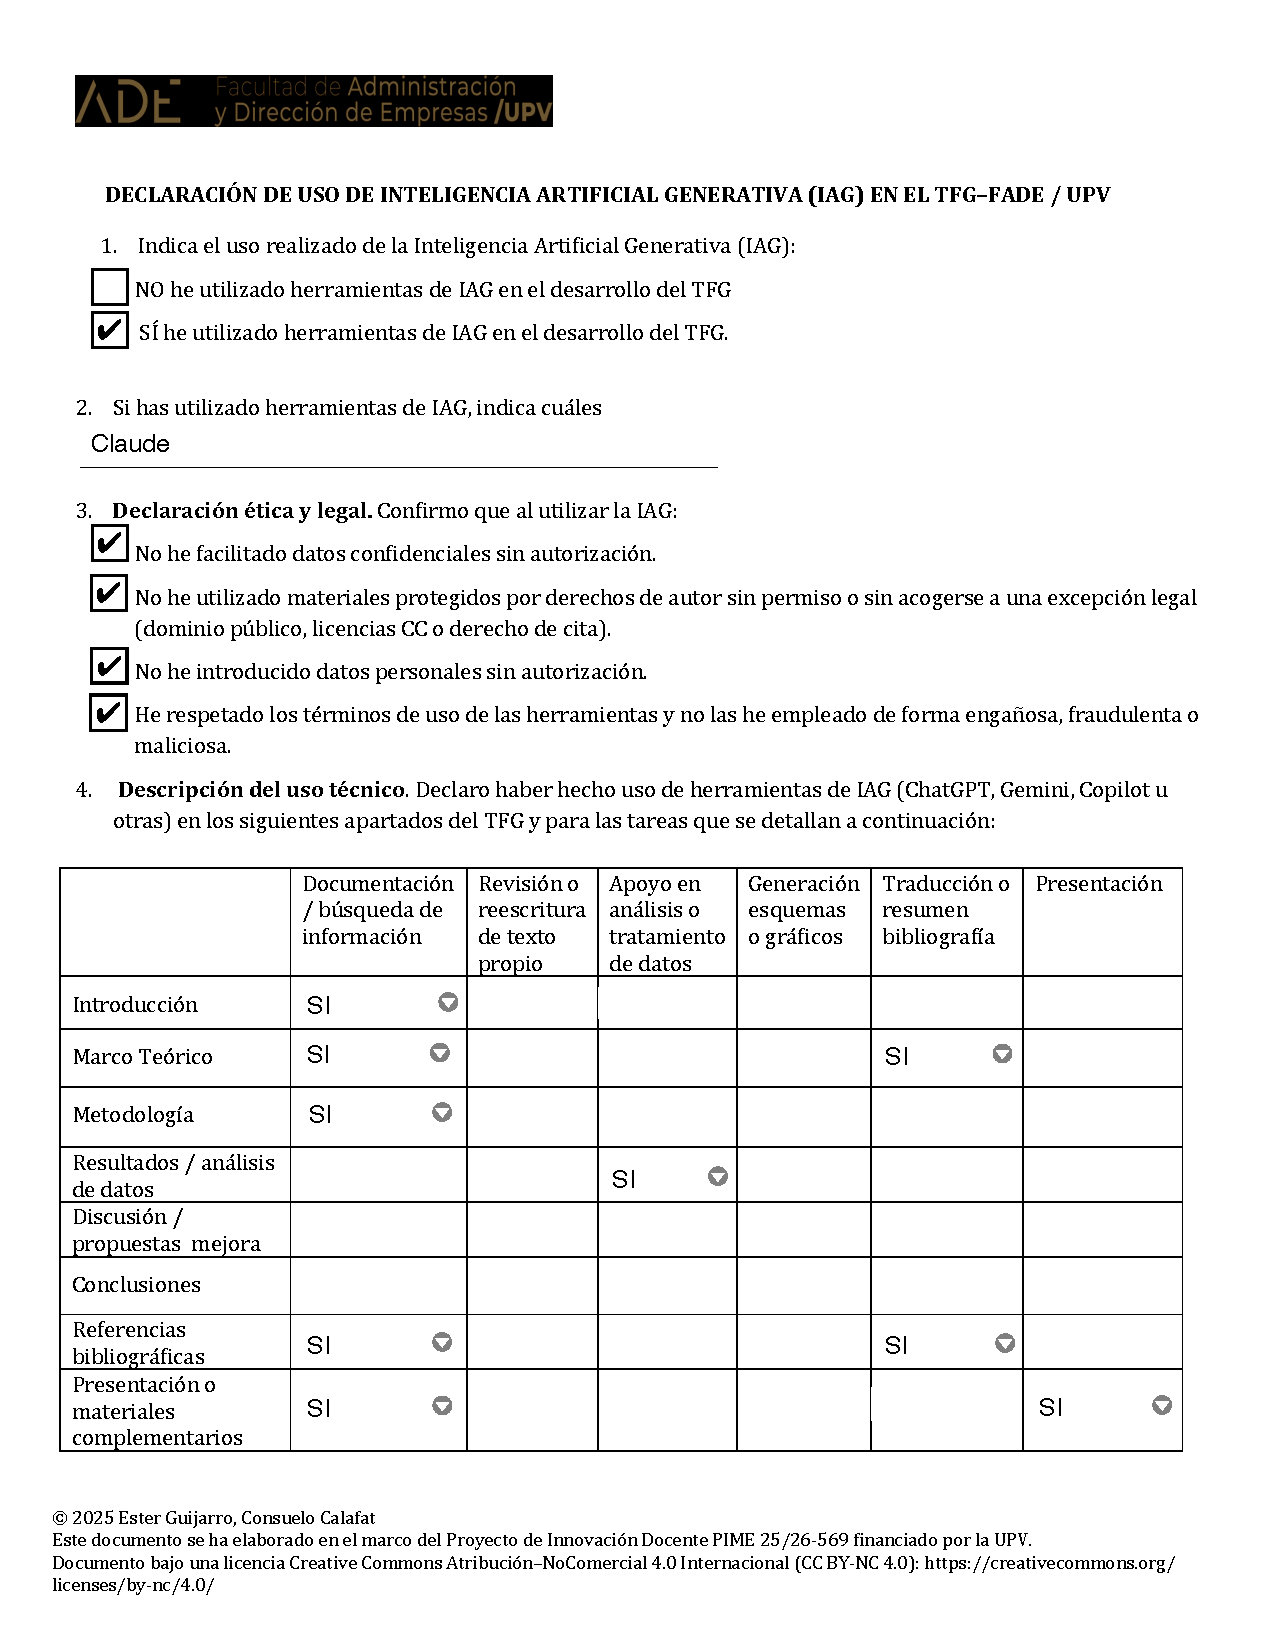
\includepdf[pages=-]{../../Declaracion_Uso_IA_TFG_FADE_UPV_v2.pdf}
